\documentclass[a4paper,14pt]{extarticle}
\usepackage[utf8x]{inputenc}
\usepackage[T1,T2A]{fontenc}
\usepackage[russian]{babel}
\usepackage{hyperref}
\usepackage{indentfirst}
\usepackage{listings}
\usepackage{color}
\usepackage{here}
\usepackage{array}
\usepackage{multirow}
\usepackage{graphicx}

%\usepackage{mathptmx}

%% Переименование "содержания" в "оглавление"
\renewcommand\contentsname{Оглавление}
\renewcommand\refname{Список использованных источников}

\bibliographystyle{ugost2008ls}

\usepackage{caption}
\renewcommand{\lstlistingname}{Программа} % заголовок листингов кода

\usepackage{listings}
\lstset{ %
extendedchars=\true,
keepspaces=true,
language=bash,					% choose the language of the code
basicstyle=\footnotesize,		% the size of the fonts that are used for the code
numbers=left,					% where to put the line-numbers
numberstyle=\footnotesize,		% the size of the fonts that are used for the line-numbers
stepnumber=1,					% the step between two line-numbers. If it is 1 each line will be numbered
numbersep=5pt,					% how far the line-numbers are from the code
backgroundcolor=\color{white},	% choose the background color. You must add \usepackage{color}
showspaces=false				% show spaces adding particular underscores
showstringspaces=false,			% underline spaces within strings
showtabs=false,					% show tabs within strings adding particular underscores
frame=single,           		% adds a frame around the code
tabsize=2,						% sets default tabsize to 2 spaces
captionpos=b,					% sets the caption-position to bottom
breaklines=true,				% sets automatic line breaking
breakatwhitespace=false,		% sets if automatic breaks should only happen at whitespace
escapeinside={\%*}{*)},			% if you want to add a comment within your code
postbreak=\raisebox{0ex}[0ex][0ex]{\ensuremath{\color{red}\hookrightarrow\space}}
}

%% Полуторный интервал
\usepackage[nodisplayskipstretch]{setspace}
\onehalfspacing

\usepackage[a4paper,includefoot,includehead,left=2.5cm,right=1.8cm,
top=2cm,bottom=2.5cm,bindingoffset=0cm]{geometry}


%% Выравнивание номара страницы по правому краю
\usepackage{fancyhdr}
\pagestyle{fancy}
\fancyhf{}
\protect\fancyfoot[R]{\thepage}
\renewcommand{\headrulewidth}{0pt}
\renewcommand{\footrulewidth}{0pt}

%% Нумерация картинок по секциям
\usepackage{chngcntr}
\counterwithin{figure}{section}
\counterwithin{table}{section}

%% Поля подписи и даты
\newcommand{\sign}[1][5cm]{%
\makebox[#1]{\hrulefill}
}

%% Количесво рисунков
\usepackage{totcount}
\newtotcounter{citenum}
\def\oldcite{}
\let\oldcite=\bibcite
\def\bibcite{\stepcounter{citenum}\oldcite}

\usepackage[figure,table,lstlisting]{totalcount}
% страниц
\usepackage{lastpage}
% библиографий
\newtotcounter{citnum} %From the package documentation
\def\oldbibitem{} \let\oldbibitem=\bibitem
\def\bibitem{\stepcounter{citnum}\oldbibitem}
% листингов (подключённых)
\newtotcounter{listnum}
\def\oldlstinputlisting{} \let\oldlstinputlisting=\lstinputlisting
\def\lstinputlisting{\stepcounter{listnum}\oldlstinputlisting}

%% Добавление промежуточных точек в оглавление
\usepackage{tocloft}
\renewcommand{\cftsecdotsep}{\cftdotsep}
\renewcommand{\cftsecleader}{\cftdotfill{\cftsecdotsep}}

%%Точки нумерации заголовков
\usepackage{titlesec}
\titlelabel{\thetitle.\quad}
\usepackage[dotinlabels]{titletoc}

%% Оформления подписи рисунка
\addto\captionsrussian{\renewcommand{\figurename}{Рисунок}}
\captionsetup[figure]{labelsep = period}

%% Подпись таблицы
\DeclareCaptionFormat{hfillstart}{\hfill#1#2#3\par}
\captionsetup[table]{format=hfillstart,labelsep=newline,justification=centering,skip=-10pt,textfont=bf}



\begin{document}	% начало документа
\counterwithin{lstlisting}{section}

% Титульная страница
%\begin{titlepage}	% начало титульной страницы

	\begin{center}		% выравнивание по центру

		Санкт-Петербургский Политехнический Университет Петра Великого\\
		Институт компьютерных наук и технологий \\
		Кафедра компьютерных систем и программных технологий\\[3cm]
		% название института, затем отступ 6см
		
		\huge \textbf{КУРСОВАЯ РАБОТА}\\[0.5cm]
		\large Дисциплина: Администрирование компьютерных сетей\\[0.1cm]
		\large Тема работы: Создание и настройка компьютерной сети для издательской фирмы\\[2cm]

	\end{center}


	\begin{flushright} % выравнивание по правому краю
%		\begin{minipage}{0.5\textwidth} % врезка в половину ширины текста
%			\begin{flushleft} % выровнять её содержимое по левому краю

				\large Выполнил студент группы 13541/4\\
				\large Зорин А. Г.\\[0.5cm]
				
				\large Преподавтель: доцент\\
				\sign[4cm]\large Малышев И. А.\\
				«\underline{\hspace{0.7cm}}» \underline{\hspace{2cm}} \the\year г.

%			\end{flushleft}
%		\end{minipage}
	\end{flushright}
	
	\vfill % заполнить всё доступное ниже пространство

	\begin{center}
	\large Санкт-Петербург\\
	\large \the\year % вывести дату
	\end{center} % закончить выравнивание по центру

\thispagestyle{empty} % не нумеровать страницу
%\end{titlepage} % конец титульной страницы
\newpage


% Содержание
% Содержание
\renewcommand\contentsname{\centerline{Содержание}}
\tableofcontents
\thispagestyle{fancy}
\newpage



\section{Цель работы}
Целю данного проекта является создание и настройка компьютерной сети для издательской фирмы средствами VMware Workstation. Установка и конфигурация необходимых сервисов. Устанавливаемые сервисы можно разделить на два типа:
\begin{itemize}  
\item Общие сервисы, необходимые для конфигурации сети 
\begin{itemize}
\item DNS сервер - для создания собственной зоны и расширения имен
\item DHCP сервер - для автоматического получения настроек сети
\end{itemize}
\item Специализированные сервисы, необходимые для корректно работы издательской фирмы
\begin{itemize}
\item FTP сервер - для обеспечения возможности удобного обмена информцией между сотрудниками  
\item Mail - создание публичных и доступных аккаунтов для всех сотрудников
\item Jenkins CI - для сборки tex файлов
\end{itemize}
\end{itemize}

\section{Создание и конфигурирование сети}
Топология создаваемой сети приведена на рисунке 1. Данный рисунок, в том числе, показывает, на каких машинах будет установлен тот или иной сервис. Основная сеть разделена на три подсети:
\begin{itemize}
\item VMNet8 - сеть с NAT сервером для выхода в интерент
\item VMNet1 - основная сеть, в которой расположен маршрутизатор, сервера и локальные машины сотрудников
\end{itemize}

\begin{figure}[H]
	\begin{center}
		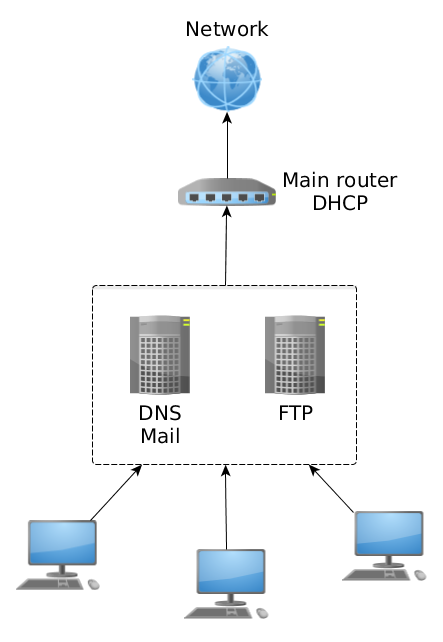
\includegraphics[width=0.6\linewidth]{pics/topology}
		\caption{Топология сети}
		\label{fig:topology}
	\end{center}
\end{figure}

В зависимости от предназначения машины, выбирается соответствующе ОС:
\begin{itemize}
\item NetBSD - для маршрутизатора
\item Ubuntu Server - для серверов
\item Ubuntu - для локальных машин
\end{itemize}

Приступим к рассмотрению процесса конфигурации

\subsection{Настройка NetBSD}
Для осуществления настройки машины с ОС NetBSD необходимо указать настройки каждого интерфейса в файле /etc/rc.conf, разрешить ip-forwarding в /etc/sysctl.conf и прописать настройки трансляции адресов в /etc/ipnat.rule (рис. 2). 

\begin{figure}[H]
	\begin{center}
		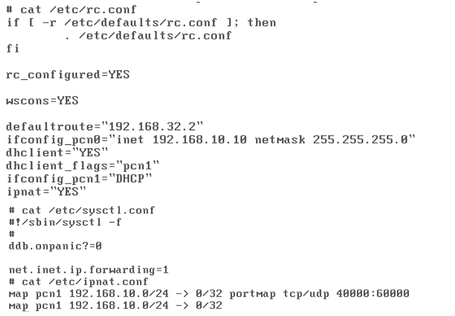
\includegraphics[width=0.6\linewidth]{pics/netBSD}
		\caption{Конфигурация NetBSD}
		\label{fig:NetBsd}
	\end{center}
\end{figure}

\subsection{Настройка Ubuntu Server}
Все сервера должны иметь статические IP-адреса. Для их настройки необходимо отредактировать файл /etc/network/interfaces. Для статического IP указываем слежующие настройки. Указанные настройки идентичны для каждого сервера. Различаются только адреса. 
\lstinputlisting[label=code:hello]{listings/ubuntuServer}

\subsection{Настройка клиентской Ubuntu}
Для корректного получения настроек по сети, на пользовательской машине достаточно будет настроить работу с DHCP.
\lstinputlisting[label=code:hello]{listings/ubuntu}

\section{Установка и настройка сетевых сервисов}
\subsection{Настройка DHCP}
Настройку DHCP сервера производим на маршрутизаторе с ОС NetBSD. Настройки DHCP сервера находятся в фалйе /etc/dhcpd.conf. В том случае, если данного файла нет в системе, его необходимо создать. В конфигурационном файле указывается доменное имя сети, адрес DNS, и настройки для сети.\\
Если все настройки заданы верно, то при включении DHCP на клиентской машине, будут выданы IP-адрес из указанного диапазона, шлюз по умолчанию и адрес DNS сервера (рис. ).

\subsection{Настройка DNS}
Настройка DNS производится на сервере с ОС Ubuntu Server и IP-адресом: 192.168.10.7. Для выполнения этой задачи необходимо установить DNS сервер BIND9. Данный сервер доступен из репозитриев Ubuntu. Следовательно, для его установки будет достаточно команды:\textit{sudo apt install bind9}.
После установки, приступаем непосредственно к конфигурации сервера. Основные его настройки находятся в файле \textit{/etc/named.conf}:
\lstinputlisting[label=code:hello]{listings/bind9}

Единственное изменение, внесенное в данный файл - объявление своей зоны \textit{example.com}. В этом файле мы указали, что данный сервер будет мастер-сервером для этой зоны и указали путь к файлу с описанием этой зоны. Ниже покажем содержание данного файла:
\lstinputlisting[label=code:hello]{listings/dns}

В данном файле, помимо стандартных записей были указаны:
\begin{itemize}
	\item ftp.example.com - ftp сервер (192.168.10.8)
	\item mail.example.com - почтовый сервер (192.168.10.7)
	\item ci.example.com - jenkins (192.168.10.8)
\end{itemize}
Следующий этап - перезагрузка сервера DNS и добавление его в автозапуск.
\begin{lstlisting}
sudo systemctl restart named
sudo systemctl enable named
\end{lstlisting}
С клиентской машины была произведена проверка работы DNS сервера (рис. ).

\subsection{Настройка FTP}
Настройка FTP сервера необходима для возможности удобного обмена данными между сотрудниками издательской фирмы. У всех сотрудников должны быть одинаковые права доступа к информации. Одним из главных критериев организации сети в издательской фирме является безопасность. Исходя из этого критерия были осуществленны следующие настройки сервера:
\begin{itemize}
	\item Ограничение свободного доступа к серверу
	\item Обеспечение возможности записи на сервер для пользователей, вошедших на сервер
	\item Настройка SSL подключения
\end{itemize}
Настройки сервера производятся в файле \textit{/etc/vsftpd/vsftpd.conf}:
\lstinputlisting[label=code:hello]{listings/ftp}
После настройки - перезапускаем сервер и добавляем его в автозагрузку:
\begin{lstlisting}
sudo systemctl restart vsftpd
sudo systemctl enable vsftpd
\end{lstlisting}

\subsection{Настройка почтового сервера}
Установка почтового сервера произведена на машине с IP-адресом 192.168.10.7. Для достижения заданной цели был использован популярный почтовый сервер iRedMail. Данное решение представляет из себя бесплатный проект с открытым исходным кодом для различных Linux дистрибутивов. iRedMail является защищенным решением, хранение паролей производится в хэшированном виде и доступ к почтовым сервисам осуществляется через защищенное соединение.\\
Установку iRedMail можно выполнить двумя способами:
\begin{itemize}
	\item Из исходных файлов, которые находятся на \textit{bitbucket}
	\item Cкачать стабильную версию с сайта
\end{itemize}
В данной работе был использован первый способ:
\begin{lstlisting}
cd /root
wget https://bitbucket.org/zhb/iredmail/downloads/iRedMail-0.9.5-1.tar.bz2
tar -xjf iRedMail-0.9.5-1.tar.bz2
cd iRedMail-0.9.5-1
sh iRedMail.sh
\end{lstlisting}
После выполнения данных строк, запустится скрипт установки iRedMail. Во время установки необходимо будет ввести требуемые параметры, такие как используемая база данных (OpenLDAP, MySQL, PostgreSQL), аккаунт администратора, почтовый домен и т.д.\\
Когда установка завершена, в браузере можно зайти на веб-страницу администратора почты по адресу \textit{https://mail.example.com/iredadmin}.\\
Для удобного доступа сотрудников к своей почте, настроим почтовый клиент Mozilla Thunderbird и попробуем отправить с него почту на почтовый адрес в yandex.
\begin{figure}[H]
	\begin{center}
		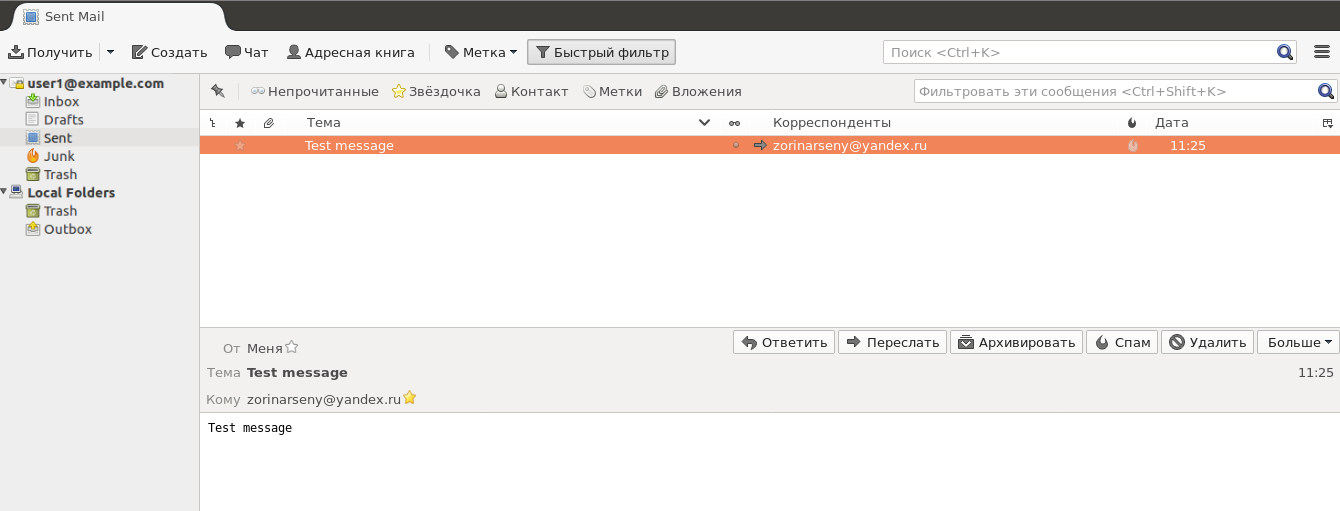
\includegraphics[width=0.6\linewidth]{pics/mail}
		\caption{Проверка работы почтового сервера}
		\label{fig:mail}
	\end{center}
\end{figure}

\subsection{Настройка Jenkins CI}
Полезным сервисом для издательской фирмы будет непрерывная сборка tex файлов. Для настройки такого сервиса был использован Jenkins. Данное решение является бесплатным с открытым исходным кодом и может использоваться для автоматизации различных задач, таких как: сборка, тестирование и развертывание программного обеспечения.
\\Установка Jenkins была произведена на той же машине, что и FTP сервер. На ОС Ubuntu Server необходимо выполнить следующие команды:
\begin{lstlisting}
wget -q -O - https://pkg.jenkins.io/debian/jenkins-ci.org.key | sudo apt-key add -
sudo sh -c 'echo deb http://pkg.jenkins.io/debian-stable binary/ > /etc/apt/sources.list.d/jenkins.list'
sudo apt update
sudo apt install jenkins
\end{lstlisting}
Данные команды устанавливают Jenkins и, в последующем, он будет запускаться в виде демона на старте системы. По умолчанию Jenkins запускается по адресу \texit{http://localhost:8080/}. Для того, чтобы можно было получить доступ к Jencins по адресу \texit{ci.example.com}, необходимо настроить nginx. Сначала необходимо его установить и удалить стандартные настройки:
\begin{lstlisting}
sudo aptitude -y install nginx
cd /etc/nginx/sites-available
sudo rm default ../sites-enabled/default
\end{lstlisting}

Создаем свои настройки и указываем ci.example.com.
\lstinputlisting[label=code:hello]{listings/nginx}

Вся последующая конфигурация работы Jenkins производится с помощью вебинтерфейса.

\section*{Заключение}
\addcontentsline{toc}{section}{Заключение}
В результате выполнения работы была создана и настроена виртуальная локальная сеть издательского агенства. Работа была выполнена средствами VMwar Workstation. \\
В ходе работы были установлены и сконфигурированы различные сервисы такие, как обычные сервисы, необходимые для корректной работы сети, так и специализированные. 
Для настройки DNS сервера был использован BIND9. Была создана своя зона \textit{example.com} и база соответствия доменных имен IP-адресам. \\
Для снастройки FTP сервера был использован vsftpd. Данный сервер был сконфигурирован согласно требованиям, предъявляемым организации сети в издательской фирме. \\
Создание почтового сервера основывается на установке и настройке iRedMail. С установленного сервера получилось отправить сообщение на существующий почтовый ящик. \\
Последний сервис, который был настроен - Jenkins. Данный сервис позволяет организовать сборку файлов Tex. Он очень прост в настройке, так как вся настройка производится через веб-интерфейс.

\end{document}
